\section{Repaso breve de probabilidad}

La teoría de probabilidades se basa en postular un espacio
abstracto $\Omega$ en el que se ``sortea'' un elemento $\alpha$.
Se asigna una probabilidad $P(A)\in [0,1]$ a ciertos subconjuntos
$A\subset\Omega$, llamados ``sucesos".

Si lo aleatorio es un número real, podríamos tomar $\Omega=\R$,
pero en general se piensa en el sorteo como algo que está
``detrás" y determina el valor $X(\alpha)$ a través de una función
$X:\Omega\rightarrow\R$, llamada {\em variable aleatoria} (V.A.)

\begin{minipage}{0.3\textwidth}La función de distribución de una V.A. se define como $F_X(x)=P\left(\{X\leq x\}\right)$\end{minipage}\hfill
\begin{minipage}{0.6\textwidth}
    \resizebox{\textwidth}{!}{
    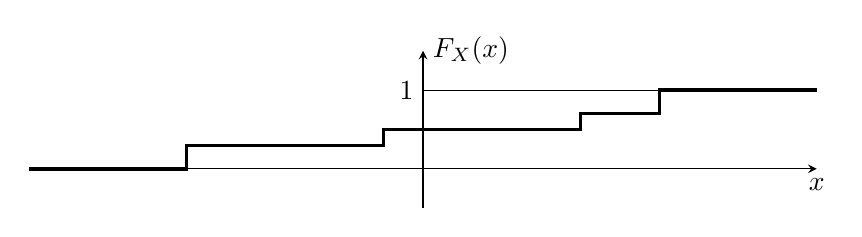
\begin{tikzpicture}
        \draw [-stealth] (-5,0) -- (5,0) node [anchor=north] {$x$};
        \draw [-stealth] (0,-0.5) -- (0,1.5) node [anchor=west] {$F_X(x)$};
        \draw [very thin] (0,1) node [anchor=east] {$1$} -- (5,1);
        \draw [very thick] (-5,0) -- (-3,0) -- (-3,0.3) -- (-0.5,0.3) -- (-0.5,0.5) -- (2,0.5) -- (2,0.7) -- (3,0.7) --  (3,1) -- (5,1);
    \end{tikzpicture}}
\end{minipage}

$F_X(x)$ está entre $0$ y $1$, es monótona creciente y continua a
la derecha.

\begin{ejemplo}
    \back
Variable aleatoria discreta.\\
    \begin{minipage}{0.3\textwidth}
        $X$ toma sólo los valores $\{x_1, \ldots, x_N\}$.
    \end{minipage}\hfill
    \begin{minipage}{0.6\textwidth}
    \resizebox{\textwidth}{!}{
    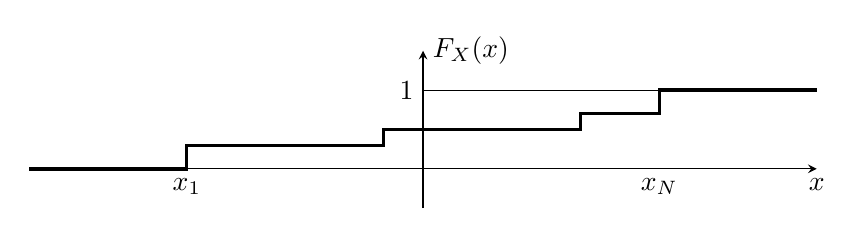
\begin{tikzpicture}
        \draw [-stealth] (-5,0) -- (5,0) node [anchor=north] {$x$};
        \draw [-stealth] (0,-0.5) -- (0,1.5) node [anchor=west] {$F_X(x)$};
        \draw [very thin] (0,1) node [anchor=east] {$1$} -- (5,1);
        \draw [very thick] (-5,0) -- (-3,0) -- (-3,0.3) -- (-0.5,0.3) -- (-0.5,0.5) -- (2,0.5) -- (2,0.7) -- (3,0.7) --  (3,1) -- (5,1);
        \path (-3,0) node [anchor=north] {$x_1$} -- (3,0) node [anchor=north] {$x_N$};
    \end{tikzpicture}}

    Cada salto es $p_i=P(X=x_i)$.
    \end{minipage}
\end{ejemplo}

\begin{ejemplo}
    Variable aleatoria absolutamente continua, $\exists\, f_X(x)=\frac{\d{}}{\d{} x}F_X(x)$ densidad.
    \begin{figure}[htb]
        \hfil
        \bpgf{Imagenes/prob/prob-3}
        \begin{tikzpicture}[xscale=0.7]
            \draw [-stealth] (-5,0) -- (5,0) node [anchor=north] {$x$};
            \draw [-stealth] (0,-0.5) -- (0,1.5) node [anchor=west] {$F_X(x)$};
            \draw [dotted] (-5,1) -- (0,1) node [anchor=south east] {$1$} -- (5,1);
            \draw [samples=2000,domain=-4.5:4.5] plot (\x,{rad(atan(\x))/(pi)+0.5});
        \end{tikzpicture}
        \endpgfgraphicnamed
        \hfill
        \bpgf{Imagenes/prob/prob-4}
        \begin{tikzpicture}[xscale=0.7]
            \draw [-stealth] (-5,0) -- (5,0) node [anchor=north] {$x$};
            \draw [-stealth] (0,-0.5) -- (0,1.5) node [anchor=west] {$f_X(x)$};
            \draw [samples=2000,domain=-4.5:4.5] plot (\x,{1/(1+(\x)^2)});
        \end{tikzpicture}
        \endpgfgraphicnamed
        \hfil
    \end{figure}
    \FloatBarrier

    \[P(a<X\leq b) = F_X(b)-F_X(a) = \int_a^b f_X(x)\d x.\]
\end{ejemplo}

\paragraph{Nota:} Se puede definir una densidad para las V.A. discretas si se
aceptan en ella $\delta$'s de Dirac. Es decir, en este caso \[
 f_X(x)=\sum_i p_i \delta(x-x_i).\]
 Esta convención se adopta en lo que sigue.

\subsection*{Valor esperado de una variable aleatoria}
\[
E[X] =\int_{-\infty}^\infty x f_X(x)\d x. \]

Representa el promedio ponderado por la probabilidad. Notar que en
el caso de las V.A. discretas, lo anterior equivale a
$E[X]=\sum_i x_ip_i$.

{\bf Momento de orden k}
\[E[X^k]=\int_{-\infty}^\infty x^kf_X(x)\d x. \]

{\bf Varianza:}  $\var[X]=E[X^2]-E[X]^2$.

\begin{ejemplo}
    V.A. Gaussiana,
    \[f_X(x)=\frac{1}{\sqrt{2\pi}\sigma}\e^{-\frac{(x-\mu)^2}{2\sigma^2}}; \quad  E[X]=\mu, \qquad
    \var[X]=\sigma^2.\]
\end{ejemplo}

Distribución {\em conjunta} de $n$ variables aleatorias $X_1,
X_2,\ldots, X_n$:

\[F_{X_1,\ldots,X_n}(x_1,x_2,\ldots,x_n)=P\left(\{X_1\leq x_1,\ldots, X_n\leq x_n\}\right).\]

\subsection*{Independencia}

\begin{itemize}
    \item 2 sucesos $A,B\subset\Omega$ son independientes si $P(A\cap
    B)=P(A)P(B)$.
    \item 2 V.A. $X$, $Y$, son independientes si los sucesos $\{X\leq x\}, \{Y\leq y\}$
    son independientes, es decir
    \begin{align*}
                                           % \underbrace{)} & = P(X\leq x)P(Y\leq y)\\
                                            F_{XY}(x,y) & = F_X(x)
                                            F_Y(y).
                                        \end{align*}
\end{itemize}

\paragraph{Propiedad: } Si $X,Y$ independientes $\Rightarrow \ \ E[XY]=E[X]E[Y]$.

Este valor esperado también es una forma de \emph{correlación}. Si
$X(\alpha)$ e $Y(\alpha)$ se ``acompañan'', $E[XY]$ da grande.
$\langle X,Y\rangle=E[XY]$ es un producto interno entre V.A. de
$E[X^2]$ finito.

La \emph{covarianza} de 2 V.A. se define como
$E\left[\left(X-E[X]\right)\left(Y-E[Y]\right)\right]=E[XY]-E[X]E[Y]$.
Si $X,Y$ independientes, entonces $\mathrm{Cov}(X,Y)=0$. Se dice
que están no correlacionadas. El recíproco no vale en general, sí
para V.A. Gaussianas.
